% chktex-file 1
% chktex-file 2
% chktex-file 3
% chktex-file 8
% chktex-file 9
% chktex-file 12
% chktex-file 13
% chktex-file 16
% chktex-file 18
% chktex-file 24
% chktex-file 26
% chktex-file 35
% chktex-file 44
% chktex-file 45

\documentclass[]{article}
\usepackage[utf8]{inputenc}
\usepackage[english]{babel}

\usepackage[]{csvsimple}
\usepackage{float}

\usepackage{ragged2e}
\usepackage[left=25mm, right=25mm, top=15mm]{geometry}
\geometry{a4paper}
\usepackage{graphicx}
\usepackage{booktabs}
\usepackage{paralist}
\usepackage{subfig} 
\usepackage{fancyhdr}
\usepackage{amsmath}
\usepackage{amssymb}
\usepackage{amsfonts}
\usepackage{amsthm}
\usepackage{mathtools}
\usepackage{enumitem}
\usepackage{titlesec}
\usepackage{braket}
\usepackage{gensymb}
\usepackage{url}
\usepackage{hyperref}
\usepackage{csquotes}
\usepackage{multicol}
\usepackage{graphicx}
\usepackage{wrapfig}
\usepackage{babel}
\usepackage{caption}
\captionsetup{font=small}
\pagestyle{fancy}
\renewcommand{\headrulewidth}{0pt}
\lhead{}\chead{}\rhead{}
\lfoot{}\cfoot{\thepage}\rfoot{}
\usepackage{sectsty}
\usepackage[nottoc,notlof,notlot]{tocbibind}
\usepackage[titles,subfigure]{tocloft}
\renewcommand{\cftsecfont}{\rmfamily\mdseries\upshape}
\renewcommand{\cftsecpagefont}{\rmfamily\mdseries\upshape}

\let\oldsection\section% Store \section
\renewcommand{\section}{% Update \section
	\renewcommand{\theequation}{\thesection.\arabic{equation}}% Update equation number
	\oldsection}% Regular \section
\let\oldsubsection\subsection% Store \subsection
\renewcommand{\subsection}{% Update \subsection
	\renewcommand{\theequation}{\thesubsection.\arabic{equation}}% Update equation number
	\oldsubsection}% Regular \subsection

\newcommand{\abs}[1]{\left\lvert#1\right\rvert}
\newcommand{\norm}[1]{\left\lVert#1\right\rVert}

\newcommand{\g}{\text{g}}
\newcommand{\m}{\text{m}}
\newcommand{\cm}{\text{cm}}
\newcommand{\mm}{\text{mm}}
\newcommand{\s}{\text{s}}
\newcommand{\N}{\text{N}}
\newcommand{\Hz}{\text{Hz}}

\newcommand{\virgolette}[1]{``\text{#1}"}
\newcommand{\tildetext}{\raise.17ex\hbox{$\scriptstyle\mathtt{\sim}$}}


\renewcommand{\arraystretch}{1.2}

\addto\captionsenglish{\renewcommand{\figurename}{Fig.}}
\addto\captionsenglish{\renewcommand{\tablename}{Tab.}}

\DeclareCaptionLabelFormat{andtable}{#1~#2  \&  \tablename~\thetable}


\title{%
    \Huge Interferometro di Michelson \\
    \Large Laboratorio di Ottica, Elettronica e Fisica Moderna \\ C.d.L. in Fisica, a.a. 2023-2024 \\ Università degli Studi di Milano}
\author{\LARGE Lucrezia Bioni, Leonardo Cerasi, Giulia Federica Bianca Coppi \\ Matricole: 13655A, 11410A, 11823A}
\date{9 novembre 2023}

\begin{document}

\maketitle

\section{Introduzione}

\subsection{Scopo}

In questa esperienza ci si propone di misurare - mediante l'utilizzo dell'interferometro di Michelson - le seguenti quantità: la lunghezza d'onda di un fascio di luce monocromatica, l'indice di rifrazione dell'aria, la lunghezza di coerenza dei pacchetti d'onda di una sorgente non monocromatica e la separazione tra le due lunghezze d'onda del doppietto del sodio.
\subsection{Metodo}

Per la misurazione delle quattro grandezze interessate, si utilizza l'apparato sviluppato da Michelson riportato in figura:
\begin{figure}[!h]
    \centering
    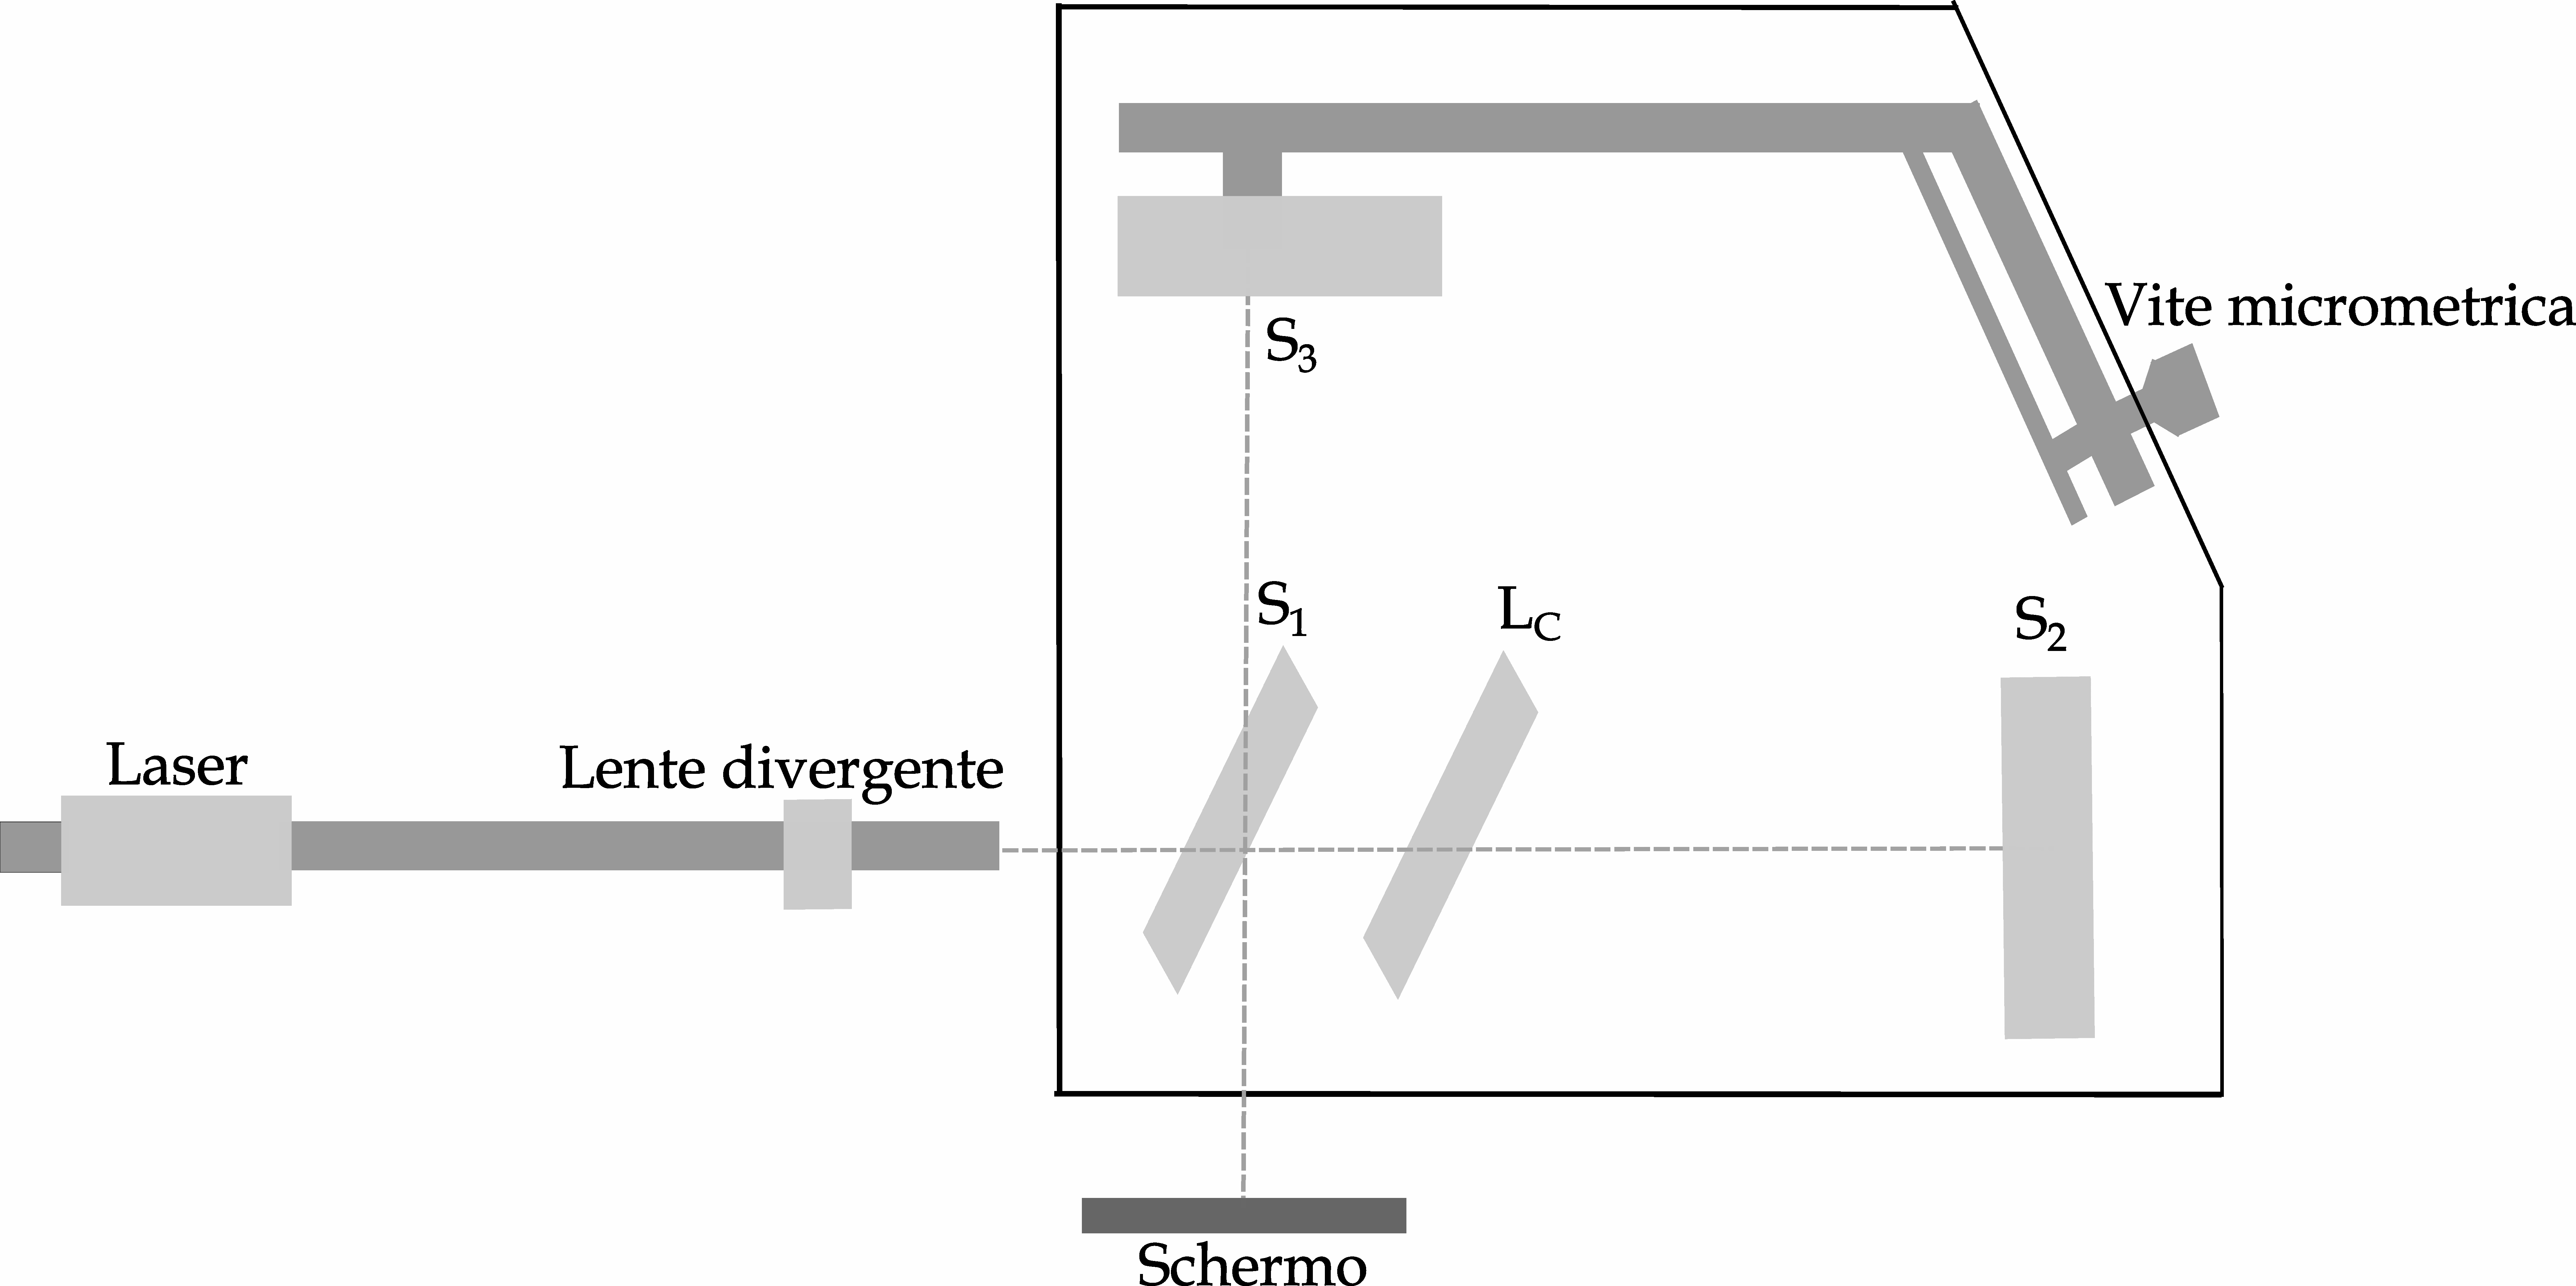
\includegraphics[width=0.70\textwidth]{disegnetto-michelson.png}
    \caption{Schema dell'interferometro di Michelson accoppiato con la sorgente di luce disposta su un banco ottico separato.}
    \label{schema}
\end{figure}\\
L'interferometro è costituito da quattro lastre di vetro ($S_1, \, S_2, \, S_3, \, L_c$): $S_1$ è semiriflettente - rivolta verso $S_2$ - a facce piane e parallele, $S_2$ ed $S_3$ sono completamente riflettenti sulla faccia rivolta verso $S_1$, $L_c$ è una lastra trasparente il cui scopo è quello di rendere uguali i cammini ottici compiuti dai raggi lungo i due bracci dello strumento. \\ Dopo aver verificato che $S_2$ ed $S_3$ siano perpendicolari e che formino un angolo di $45\degree$ con $S_1$, il raggio luminoso inciderà su $S_1$ sdoppiandosi: il primo verrà riflesso da $S_2$ e dalla faccia riflettente di $S_1$, per poi proseguire verso lo schermo, il secondo - riflesso da $S_1$ - verrà riflesso da $S_3$ ed inciderà sullo schermo dove formerà delle figure di interferenza con il primo raggio - douvuta alla coerenza dei due fasci luminosi.

\subsubsection{Lunghezza d'onda di un fascio di luce monocromatica}

Si vuole misurare la lunghezza d'onda di un fascio di luce laser. Agendo sulla variazione di cammino ottico dei due fasci - spostando lo specchio $S_3$ - si conta il numero di frange chiare (o scure) passanti per un punto prefissato dello schermo. La misura della lunghezza d'onda è pertanto data dall'equazione:
\begin{equation}
    \label{lambda_laser}
    \lambda = \frac{2 n_a \Delta x}{N_1}
\end{equation}
dove $\lambda$ è la lunghezza d'onda incognita, $n_a$ è l'indice di rifrazione dell'aria, $\Delta x$ è lo spostamento dello specchio $S_3$ ed $N_1$ è il numero di frange chiare (o scure) contate.

\subsubsection{Indice di rifrazione dell'aria}

Tra gli specchi $S_1$ ed $S_2$ viene inserita una cameretta contenente una pompa per la creazione del vuoto. Il cammino ottico percorso dal fascio luminoso nel vuoto cambia, poichè questo è legato all'indice di rifrazione del mezzo che attraversa come mostrato dall'equazione \ref{lambda_laser}. Quindi, facendo rientrare lentamente l'aria nella cameretta e contando le frange di interferenza passanti per un dato punto sullo schermo, si riuscirà a fornire una stima del valore dell'indice di rifrazione dell'aria $n_a$ secondo la seguente equazione:
\begin{equation}
    \label{n_a}
    2(n_a - 1) = N_2 \lambda
\end{equation}
dove $n_a$ è l'indice di rifrazione dell'aria, $N_2$ è il numero di frange contate su un punto dello schermo e $\lambda$ è la lunghezza d'onda del fascio emesso dalla sorgente monocromatica.

\subsubsection{Lunghezza dei pacchetti d'onda di una sorgente non monocromatica}
\label{par:123}

Il fascio di luce prodotto da una sorgente non monocromatica è costituito da impulsi di lunghezza limitata. L'inferferenza dei fasci luminosi riflessi dagli specchi $S_2$ ed $S_3$ si manifesta quando la distanza tra le due sorgenti immagine è inferiore alla lunghezza del pacchetto. Quando viene superata tale lunghezza, si osserva sullo schermo una figura uniformemente illuminata. Dunque, si misura la distanza tra due zone di uniforme illuminazione - mediante la misura dello spostamento di $S_3$ - per quantificare tale grandezza.

\subsubsection{Differenza tra le lunghezze d'onda del doppietto del sodio}

Si utilizza ora una sorgente luminosa al sodio per misurare le due lunghezze d'onda che emette e la loro conseguente separazione. Quando le frange di interferenza delle due lunghezze d'onda si vanno a sovrapporre, sullo schermo si vede una figura di interferenza con frange molto nette - in particolare quando la differenza di cammino ottico tra i fasci provenieni da $S_2$ ed $S_3$ è nulla. 
Si misura quindi lo spostamento dello specchio $S_3$ e si ricava:
\begin{equation}
    \label{Delta_lambda}
    \lambda _2 - \lambda _1 = \frac {m \bar{\lambda} ^2 }{2 \Delta x}
\end{equation}
dove $\lambda _1$ e $\lambda _2$ sono le due lunghezze d'onda del doppietto del sodio, $m$ è il numero di alternanze tra le condizioni di interferenza netta, $\bar{\lambda}$ è la media delle due lunghezze d'onda e $\Delta x$ è lo spostamento dello spcchio $S_3$.

\section{Misure}

\subsection {Lunghezza d'onda di un fascio di luce monocromatica}

La misura della lunghezza d'onda del fascio laser viene effettuata prendendo 5 misure dello spostamento dello specchio mobile e contando le frange passanti per un punto fissato dello schermo. Le misure effettuate sono riportate nella seguente Tabella:

\begin{table}[H]
    \centering

    \begin{tabular}{||c|c|c||}
        \hline
        $N_1 $ & $x_1 \, \text{[mm]}$ & $x_2\, \text{[mm]}$ \\
        \hline\hline

        $195$ & $10.00$ & $10.30$ \\\hline
        $194$ & $10.00$ & $10.30$ \\\hline
        $150$ & $10.00$ & $10.23$ \\\hline
        $150$ & $10.00$ & $10.23$ \\\hline
        $180$ & $10.00$ & $10.28$ \\\hline
    
    \end{tabular}
    \caption{Misure di $N_1$, $x_1$ e $x_2$ effetuate per valutare la lunghezza d'onda della sorgente laser}
    \label{lambda}    
\end{table}
Al conteggio $N_1$ viene fornito un errore di $ \pm 5$, a seguito di una valutazione dell'errore commesso dagli sperimentatori; mentre alle misure di $x_1$ e $x_2$ viene fornita come incertezza la risoluzione dello strumento, pari a $0.01 \, \text{mm}$. \\ Gli spostamenti $x_1$ e $x_2$ sono effettuati attraverso una vita micrometrica che permette spostamenti fini dello specchio $S_3$ pari ad $\frac{1}{5}$ di quelli impressi dallo sperimentatore. 


\subsection{Indice di rifrazione dell'aria}
\label{par:n_a}

La camera usata per creare il vuoto ha lunghezza $D=0.05 \, \text{m}$ - valore considerato senza incertezza. Fissato un punto dello schermo, durante la reimmissione dell'aria nella camera, si conta il numero di frange d'interferenza che vi passano: in 5 misurazioni di fila, si è sempre ottenuto il valore $N_2 = 42 \pm 5$.

\subsection{Lunghezza dei pacchetti d'onda di una sorgente non monocromatica}

Vengono fatte, attraverso la lettura della posizione della vite micrometrica, 6 misure dello spostamento dello specchio per valutare la lunghezza del treno di impulsi come descritto nel Paragrafo \ref{par:123}. I risultati sono riportati in tabella:

\begin{table}[H]
    \centering

    \begin{tabular}{||c|c||}
        \hline
        $x_1 \, \text{[mm]}$ & $x_2\, \text{[mm]}$ \\
        \hline\hline

        $15.58$ & $15.54$ \\\hline
        $15.58$ & $15.54$ \\\hline
        $15.57$ & $15.54$ \\\hline
        $15.57$ & $15.54$ \\\hline
        $15.57$ & $15.54$ \\\hline
        $15.57$ & $15.54$ \\\hline
    
    \end{tabular}
    \caption{Misure della posizione iniziale e finale dello specchio $S_3$}
    \label{L}    
\end{table}
A queste misure viene sempre fornita l'incertezza strumentale pari a $0.01\text{mm}$.

\subsection{Differenza tra le lunghezze d'onda del doppietto del sodio}

Per valutare la differenza $\Delta \lambda$ tra le due lunghezze d'onda emesse dal sodio, si misura, attraverso la vite micrometrica, lo spostamento che intercorre tra due posizioni di $S_3$ tali per cui si osservi un pattern di interferenza completamente diffusa. Vengono prese 8 misure dello spostamento dello specchio $S_3$, fornendo anche il numero $m$ di alternanze di interferenze nette viste sullo schermo durante lo spostamento dello specchio mobile. Le misure vengono riportate in tabella:

\begin{table}[H]
    \centering

    \begin{tabular}{||c|c|c||}
        \hline
        $m $ & $x_1 \, \text{[mm]}$ & $x_2\, \text{[mm]}$ \\
        \hline\hline

        $1$ & $16.24$ & $17.73$ \\\hline
        $1$ & $17.73$ & $19.11$ \\\hline
        $1$ & $19.11$ & $20.66$ \\\hline
        $1$ & $20.66$ & $22.07$ \\\hline
        $1$ & $22.07$ & $23.58$ \\\hline
        $1$ & $23.58$ & $24.98$ \\\hline
        $1$ & $17.72$ & $19.15$ \\\hline
        $2$ & $19.15$ & $22.17$ \\\hline
    
    \end{tabular}
    \caption{Misure di $m$, $x_1$ e $x_2$ effettuate per valutare $\Delta \lambda$ del doppietto di $Na$ }
    \label{sodio}    
\end{table}
Dove l'indice $m$ rappresenta il numero di interferenze nitide osservate tra le posizioni iniziale e finale dello specchio rilevate. L'incertezza attribuita alle misure di $x_1$ e $x_2$ è quella strumentale: $0.01 \text{mm}$.


\section{Analisi Dati}

Ogni volta che si è misurato lo spostamento $\Delta x$, si è dovuto considerare quanto osservato in precedenza: lo spostamento effettivo dello specchio $S_3$ risulta essere $\frac{1}{5}$ di quello effettuato mediante vite micrometrica. Da una propagazione dell'errore sulla singola misura di posizione, e tenuto conto del meccanismo di funzionamento dello strumento, l'incertezza risulta essere:
\begin{equation}
    \label{err-delta-x}
    \sigma_{\Delta x} = \sqrt{ \left(\frac{\sigma_{x_1}}{5}\right)^2 + \left(\frac{\sigma_{x_2}}{5}\right)^2} = 3 \, \mu \text{m}
\end{equation}

\subsection{Lunghezza d'onda di un fascio di luce monocromatica}

A partire dai dati in Tab. \ref{lambda} e approssimando l'indice di rifrazione dell'aria a $n_a \approx 1$, tramite la relazione \ref{lambda_laser}, si sono ricavati i valori di $\lambda_0$:

\begin{table}[H]
    \centering
    
    \begin{tabular}{||c||}
        \hline
        $\lambda_0 \pm \sigma_{\lambda_0} \, \left[\text{nm}\right]$ \\
        \hline\hline

        $615 \pm 33$ \\\hline
        $617 \pm 33$ \\\hline
        $613 \pm 43$ \\\hline
        $613 \pm 43$ \\\hline
        $622 \pm 36$ \\\hline
    
    \end{tabular}
    \caption{Valori della lunghezza d'onda ricavati dal set di misure.}
    \label{tab:lambda}
\end{table}
dove l'incertezza è stata attribuita mediante propagazione degli errori sulle grandezze $\Delta x$ e $N_1$ nella \ref{lambda_laser}:
\begin{equation}
\label{err-lambda}
\sigma_{\lambda_0} = \sqrt{ \left( \frac{2 \, n_a}{N_1}\right)^2 \sigma^2_{\Delta x} +  \left(\frac{2 n_a \Delta x}{N_1} \right)^2 \sigma^2_{\Delta x} }
\end{equation}
Attraverso la media ponderata dei valori di $\lambda_0$ ottenuti, si ottiene una stima della misura della lunghezza d'onda della luce laser:
\begin{equation}
\label{lambda-value}
\lambda_0 = 617 \pm 16 \, \text{nm}
\end{equation}
dove l'incertezza è quella di una media ponderata.

\subsection{Indice di rifrazione dell'aria}

A partire dalle equazioni \ref{lambda_laser} e \ref{n_a}, si possono ricavare le seguenti espressioni per $n_a$ e $\lambda_a$:
\begin{equation}
    \label{rifrazione}
    n_a = \frac{N_1 D}{N_1 D - N_2 \Delta x} \qquad
    \lambda_a = \frac{2\Delta x D}{N_1 D - N_2 \Delta x}
\end{equation}
A questo punto, incrociando i dati in Tab. \ref{lambda} con quelli riportati nel Par. \ref{par:n_a}, si ottengono i valori riportati in Tab. \ref{tab:n_a}, nella quale i valori delle incertezze sono stati ricavati tramite le relative propagazioni degli errori:
\begin{align}
    \label{rifrazione-err}
    \sigma_n &= \frac{N_1 N_2 D \Delta x}{\left(N_1 D - N_2 \Delta x\right)^2} \sqrt{\left(\frac{\sigma_{N_1}}{N_1}\right)^2 + \left(\frac{\sigma_{\Delta x}}{\Delta x}\right)^2 + \left(\frac{\sigma_{N_2}}{N_2}\right)^2 + \left(\frac{\sigma_{D}}{D}\right)^2} \\
    \sigma_{\lambda} &= \frac{\Delta x^2 D^2}{2\left(N_1 D - N_2 \Delta x\right)^2} \sqrt{\left(\frac{N_1}{\Delta x}\right)^2\left(\left(\frac{\sigma_{N_1}}{N_1}\right)^2 + \left(\frac{\sigma_{\Delta x}}{\Delta x}\right)^2\right) + \left(\frac{N_2}{D}\right)^2\left(\left(\frac{\sigma_{N_2}}{N_2}\right)^2 + \left(\frac{\sigma_{D}}{D}\right)^2\right)}
\end{align}
Il valore finale e la rispettiva incertezza di $n_a$ e $\lambda_a$ sono stati determinati tramite media ponderata:
\begin{equation}
    \label{n_a-lambda}
    n_a = 1.000259 \pm 0.000007 \qquad
    \lambda_a = 617 \pm 8 \, \text{nm}
\end{equation}

\subsection{Lunghezza dei pacchetti d'onda di una sorgente non monocromatica}
Si calcola la lunghezza di coerenza del pacchetto d'onda della sorgente attraverso la seguente relazione: $L=\Delta x$. A tale grandezza, si attribuisce incertezza mediante propagazione degli errori su $x_1$ e $x_2$. Si può inoltre ricavare l'ampiezza del pacchetto d'onda nello spazio delle frequenze: $\Delta \nu = \frac{c}{L}$, cui è stata attribuita un'incertezza sempre mediante propagazione degli errori:
\begin{equation}
    \label{sigma-nu}
    \sigma_{\Delta \nu} = \frac{c}{L^2} \sigma_L
\end{equation}
I valori di $L$ e di $\Delta \nu$ così ottenuti sono riportati nella seguente tabella:

\begin{table}[H]
    \centering
    \begin{tabular}{||c|c||}
        \hline
        $L \pm \sigma_{L} \, \left[\mu\text{m}\right]$ & $\Delta \nu \pm \sigma_{\Delta \nu} \, \left[\cdot 10^{13}\text{Hz}\right]$ \\
        \hline\hline

        $8 \pm 3$ & $4 \pm 1$ \\\hline
        $8 \pm 3$ & $4 \pm 1$ \\\hline
        $6 \pm 3$ & $5 \pm 2$ \\\hline
        $6 \pm 3$ & $5 \pm 2$ \\\hline
        $6 \pm 3$ & $5 \pm 2$ \\\hline
        $6 \pm 3$ & $5 \pm 2$ \\\hline
    
    \end{tabular}
    \caption{Valori della lunghezza di coerenza $L$ e dell'ampiezza del pacchetto d'onda nello spazio delle frequenze $\Delta \nu$ ricavati dal set di misure.}
    \label{tab:L}
\end{table}
Attraverso una media ponderata, si ottengono i valori finali per $L$ e $\Delta \nu$ e le rispettive incertezze:
\begin{equation}
    \label{L-deltanu}
    L = 7 \pm 1 \, \mu\text{m} \qquad
    \Delta\nu = 4 \pm 1 \cdot 10^{13} \, \text{Hz}
\end{equation}

\subsection{Differenza tra le lunghezze d'onda del doppietto del sodio}
Attraverso la relazione \ref{Delta_lambda}, si determina la differenza tra le due lunghezze d'onda del Na, cui è attribuita un'incertezza mediante propagazione degli errori sulla grandezza $\Delta x$:
\begin{equation}
    \label{sigma-delta-lambda}
    \sigma_{\Delta \lambda} = \frac{m \bar{\lambda}}{2 \Delta x ^2} \sigma_{\Delta x}
\end{equation}
I valori così ottenuti sono riportati nella seguente tabella:
\begin{table}[H]
    \centering
    \begin{tabular}{||c||}
        \hline
        $\Delta \lambda [\text{nm}]$ \\
        \hline\hline

        $0.583 \pm 0.006$ \\\hline
        $0.629 \pm 0.006$ \\\hline
        $0.560 \pm 0.005$ \\\hline
        $0.616 \pm 0.006$ \\\hline
        $0.575 \pm 0.005$ \\\hline
        $0.620 \pm 0.006$ \\\hline
        $0.607 \pm 0.006$ \\\hline
        $0.575 \pm 0.003$ \\\hline
    
    \end{tabular}
    \caption{Valori di $\Delta \lambda$.}
    \label{tab:delta-lambda}
\end{table}
Attraverso la media ponderata, si è ottenuto il valore finale, con la sua incertezza, della differenza di lunghezza d'onda del doppietto del sodio:
\begin{equation}
    \label{delta-lambda-value}
    \Delta \lambda = (0.587 \pm 0.002) \, \text{nm}
\end{equation}

\section{Conclusioni}
L'indice di rifrazione dell'aria ottenuto, $n_a=1.000259 \pm 0.000007$, è in accordo, entro $2 \sigma$, con il valore universalmente accettato $\bar{n}=1.000273$ (assumendo condizioni STP).

Inoltre, i due valori della lunghezza d'onda del laser, ottenuti con e senza approssimazione dell'indice di rifrazione dell'aria, sono in perfetto accordo tra loro: $\lambda_{0} = 617 \pm 16 \, \text{nm}$ e $ \lambda_{a} =616 \pm 7 \, \text{nm}$.

La lunghezza di coerenza del pacchetto di luce non monocromatica $L= 7 \pm 1 \, \mu \text{m}$ è consistente con quanto atteso: poiché la sorgente è policromatica, genera casualmente dei pacchetti non coerenti tra loro.

Infine, il valore della differenza tra le lunghezze d'onda del doppietto del sodio $\Delta \lambda = (0.587 \pm 0.002) \, \text{nm}$ è in buon accordo con il valore atteso, $\Delta \bar{\lambda} = (0.600) \text{nm}$.

\section*{Appendice}

\begin{table}[H]
    \centering
    
    \begin{tabular}{||c|c||c|c||c|c||}

        \hline
        $N_1$ & $\Delta x \pm \sigma_{\Delta x} \, [\text{mm}]$ & $N_2$ & $D \, [\text{mm}]$ & $n \pm \sigma_n$ & $\lambda \pm \sigma_{\lambda} \, [\text{nm}]$ \\
        \hline\hline

        $195$ & $0.060 \pm 0.003$ & $42$ & $0.05$ & $1.000259 \pm 0.000034$ & $616 \pm 33$ \\\hline
        $195$ & $0.060 \pm 0.003$ & $42$ & $0.05$ & $1.000259 \pm 0.000034$ & $616 \pm 33$ \\\hline
        $195$ & $0.060 \pm 0.003$ & $42$ & $0.05$ & $1.000259 \pm 0.000034$ & $616 \pm 33$ \\\hline
        $195$ & $0.060 \pm 0.003$ & $42$ & $0.05$ & $1.000259 \pm 0.000034$ & $616 \pm 33$ \\\hline
        $195$ & $0.060 \pm 0.003$ & $42$ & $0.05$ & $1.000259 \pm 0.000034$ & $616 \pm 33$ \\\hline
        \hline
        $150$ & $0.046 \pm 0.003$ & $42$ & $0.05$ & $1.000258 \pm 0.000036$ & $613 \pm 43$ \\\hline
        $150$ & $0.046 \pm 0.003$ & $42$ & $0.05$ & $1.000258 \pm 0.000036$ & $613 \pm 43$ \\\hline
        $150$ & $0.046 \pm 0.003$ & $42$ & $0.05$ & $1.000258 \pm 0.000036$ & $613 \pm 43$ \\\hline
        $150$ & $0.046 \pm 0.003$ & $42$ & $0.05$ & $1.000258 \pm 0.000036$ & $613 \pm 43$ \\\hline
        $150$ & $0.046 \pm 0.003$ & $42$ & $0.05$ & $1.000258 \pm 0.000036$ & $613 \pm 43$ \\\hline
        \hline
        $180$ & $0.056 \pm 0.003$ & $42$ & $0.05$ & $1.000261 \pm 0.000035$ & $622 \pm 44$ \\\hline
        $180$ & $0.056 \pm 0.003$ & $42$ & $0.05$ & $1.000261 \pm 0.000035$ & $622 \pm 44$ \\\hline
        $180$ & $0.056 \pm 0.003$ & $42$ & $0.05$ & $1.000261 \pm 0.000035$ & $622 \pm 44$ \\\hline
        $180$ & $0.056 \pm 0.003$ & $42$ & $0.05$ & $1.000261 \pm 0.000035$ & $622 \pm 44$ \\\hline
        $180$ & $0.056 \pm 0.003$ & $42$ & $0.05$ & $1.000261 \pm 0.000035$ & $622 \pm 44$ \\\hline
        \hline
        $194$ & $0.060 \pm 0.003$ & $42$ & $0.05$ & $1.000260 \pm 0.000034$ & $619 \pm 33$ \\\hline
        $194$ & $0.060 \pm 0.003$ & $42$ & $0.05$ & $1.000260 \pm 0.000034$ & $619 \pm 33$ \\\hline
        $194$ & $0.060 \pm 0.003$ & $42$ & $0.05$ & $1.000260 \pm 0.000034$ & $619 \pm 33$ \\\hline
        $194$ & $0.060 \pm 0.003$ & $42$ & $0.05$ & $1.000260 \pm 0.000034$ & $619 \pm 33$ \\\hline
        $194$ & $0.060 \pm 0.003$ & $42$ & $0.05$ & $1.000260 \pm 0.000034$ & $619 \pm 33$ \\\hline
        \hline
        $150$ & $0.046 \pm 0.003$ & $42$ & $0.05$ & $1.000258 \pm 0.000036$ & $613 \pm 33$ \\\hline
        $150$ & $0.046 \pm 0.003$ & $42$ & $0.05$ & $1.000258 \pm 0.000036$ & $613 \pm 33$ \\\hline
        $150$ & $0.046 \pm 0.003$ & $42$ & $0.05$ & $1.000258 \pm 0.000036$ & $613 \pm 33$ \\\hline
        $150$ & $0.046 \pm 0.003$ & $42$ & $0.05$ & $1.000258 \pm 0.000036$ & $613 \pm 33$ \\\hline
        $150$ & $0.046 \pm 0.003$ & $42$ & $0.05$ & $1.000258 \pm 0.000036$ & $613 \pm 33$ \\\hline
        
    \end{tabular}
    \caption{non so che scriverci.}
    \label{tab:n_a}
\end{table}

\end{document}